\section{Overall System Design Schema}
Figure \ref{fig:overall} shows the overall system design in detail. Each unit is described in details in its section.

\begin{figure}[hp]
    \centering
    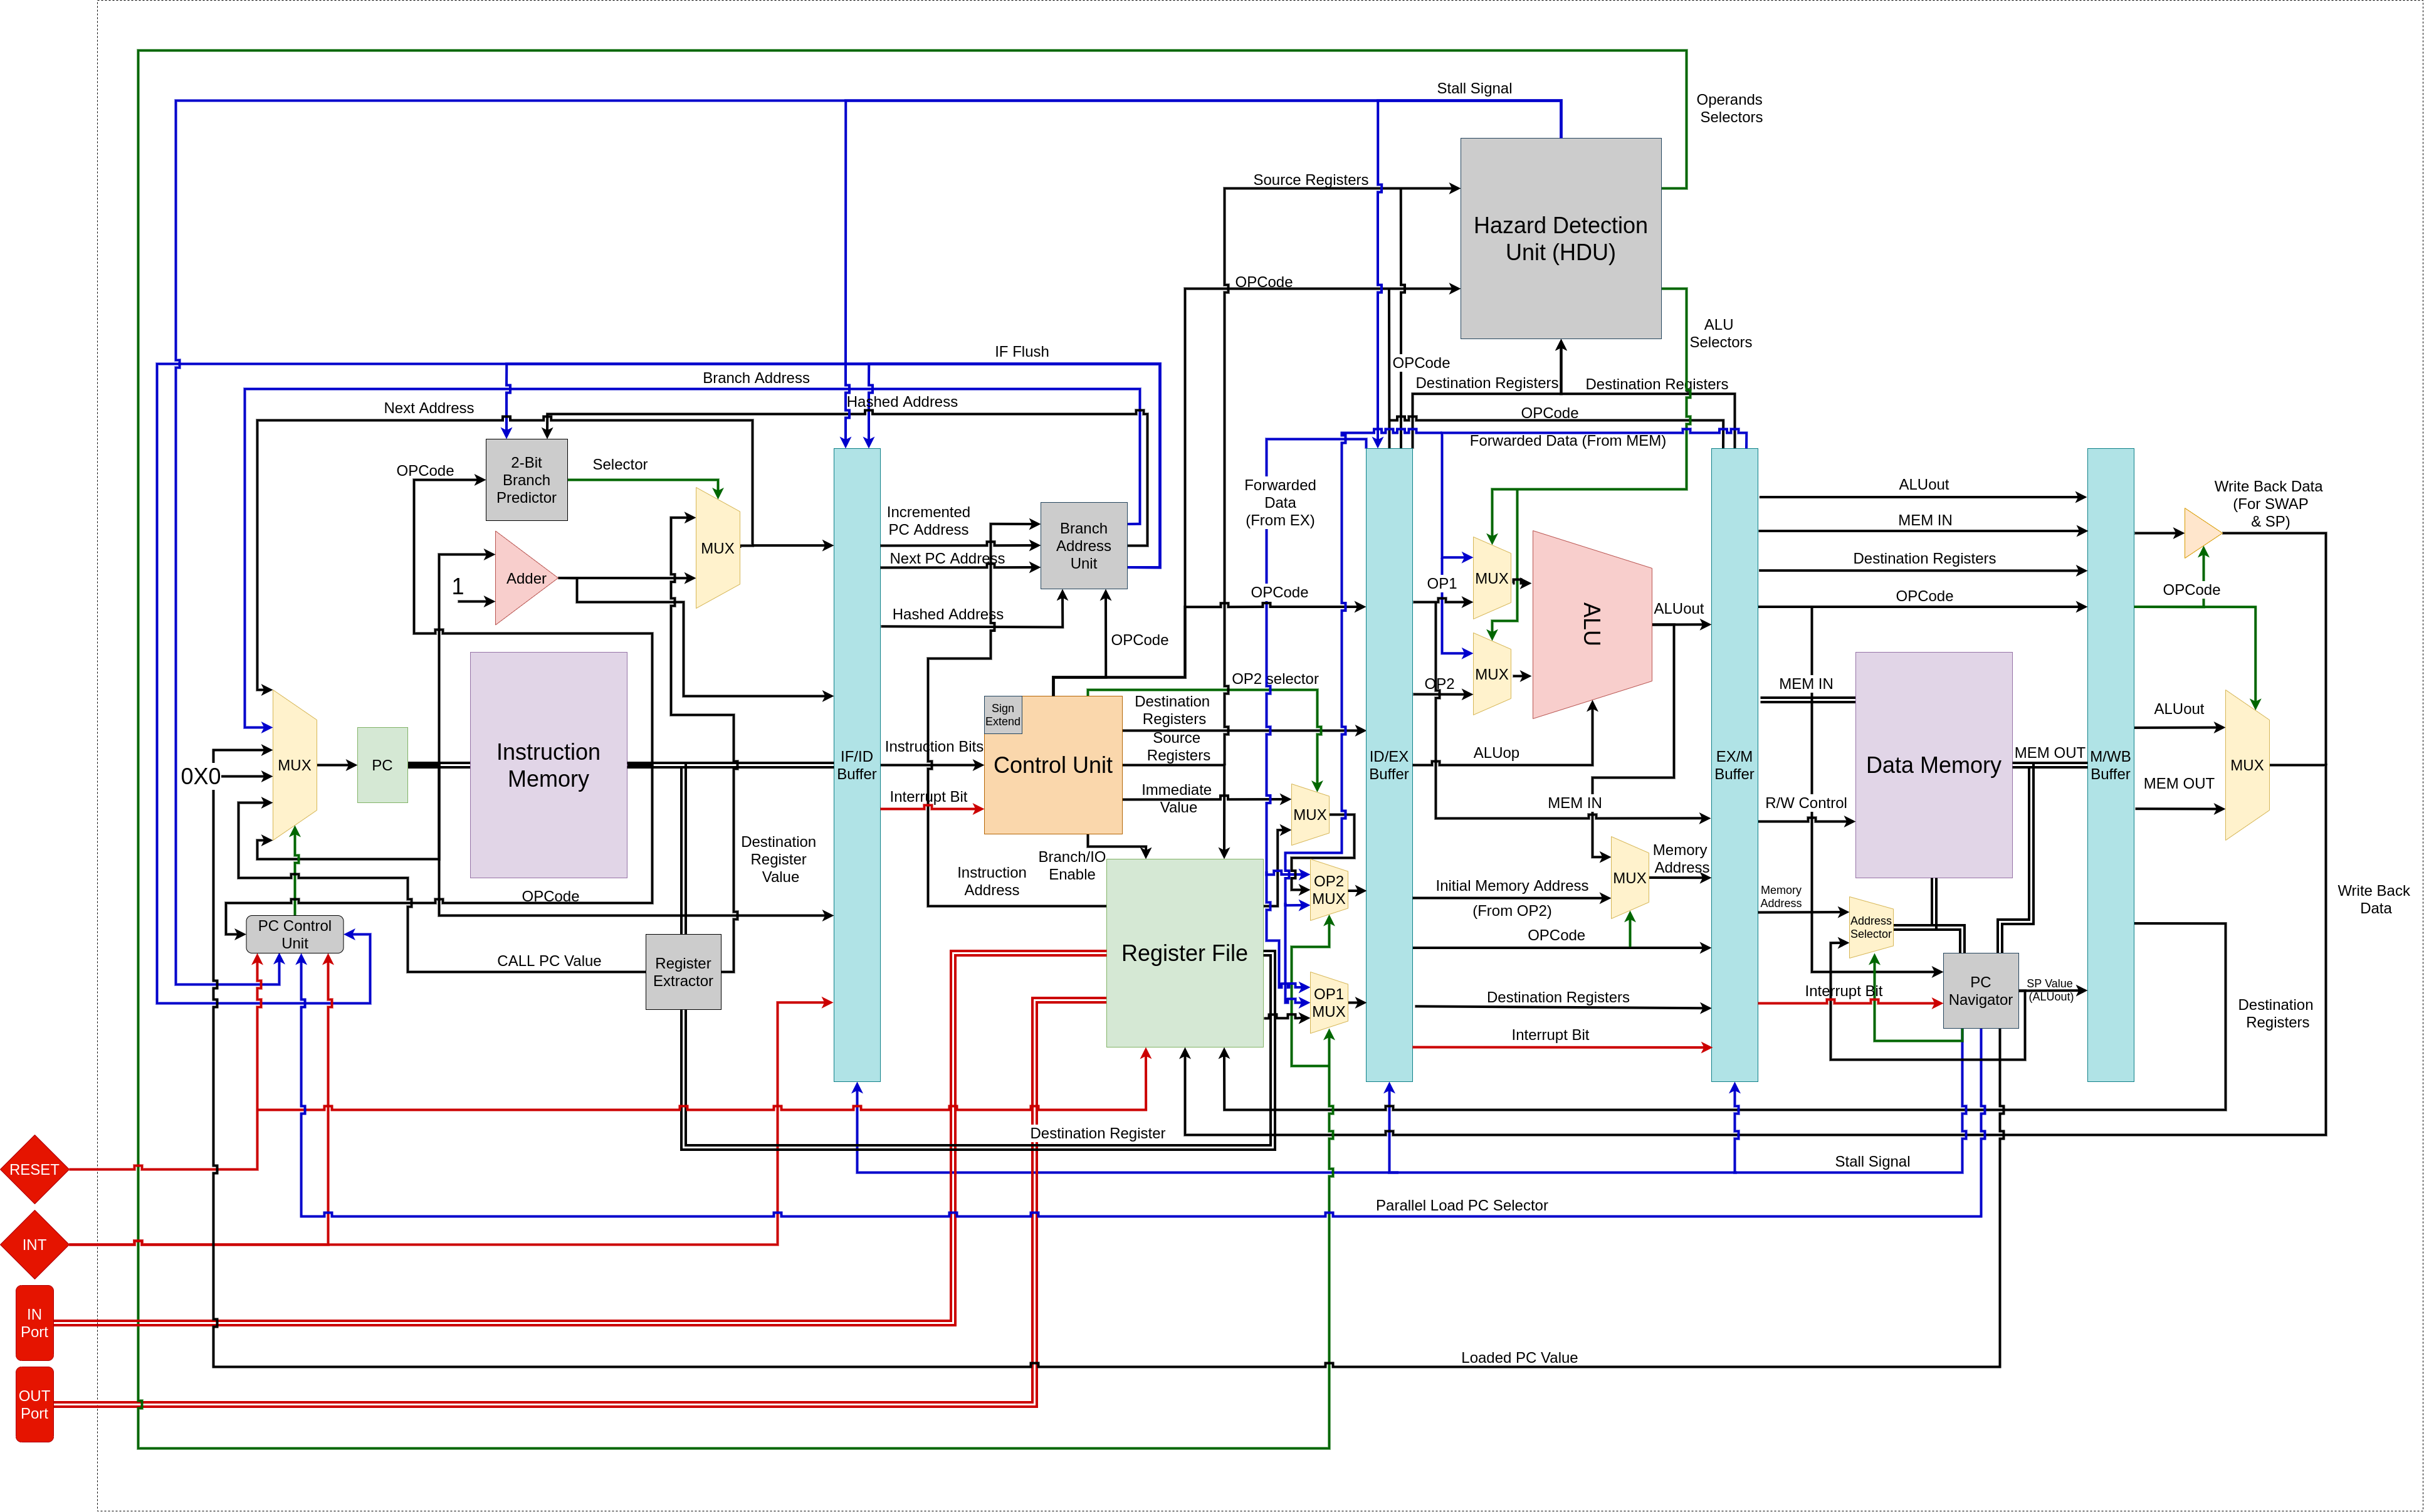
\includegraphics[width=\textwidth]{images/overall_system.png}
    \caption{Overall System Design}
    \label{fig:overall}
\end{figure}


\section{Memory Specs}
The cpu follows Harvard architecture and thus uses the following 2 separate memory units:
\begin{itemize}
    \item Instructions Memory: Read-only, stores instructions.
    \begin{itemize}
        \item \textbf{Word Width}: 16 bits.
        \item \textbf{Address Bus Width}: 8 bits.
        \item \textbf{Data Bus Width}: 16 bits.
        \item \textbf{Total Number of Words}: $2^{16}$ words = 65,536 words = 131,072 bytes.
        \item \textbf{Valid Address Range}: From 0x0000 inclusive to 0xFFFF inclusive.
    \end{itemize}
    \item Data Memory: Read-Write, stores data and the stack.
    \begin{itemize}
        \item \textbf{Word Width}: 16 bits.
        \item \textbf{Address Bus Width}: 32 bits.\\
        \textit{For simulation}, this memory will ignore bits from (31 to 10) inclusive, and only work with bits from (9 to 0) inclusive.
        \item \textbf{Data Bus Width}: 32 bits.\\
        The higher bits (31 downto 16) are data at address A~.\\
        The lower bits (15 downto 0) are data at address A+1~.\\
        where $A ~mod~ 2 = 0$~.\\
        On read, data-memory loads data bus with data from A and A+1~.\\
        On write, data-memory stores data from data bus to both A and A+1 addresses.
        \item \textbf{Total Number of Words}: $2^{32}$ words = 4,294,967,296 words = 8,589,934,592 bytes.\\
        \textit{For simulation}, this memory will only have: $2^{10}$ words = 1,024 words = 2,048 bytes.
        \item \textbf{Valid Address Range}: Even Adresses From 0x0000\_0000 inclusive to 0xFFFF\_FFFF exclusive. Formaly $A \in $[0x0000\_0000, 0xFFFF\_FFFF) and $A ~mod~ 2 = 0$~.\\
        \textit{For simulation}, range will become: Even Addresses From 0x0000\_0000 inclusive to 0x0000\_0400 exclusive. Formaly $A \in $[0x0000\_0000, 0x0000\_0400) and $A ~mod~ 2 = 0$~.
    \end{itemize}
\end{itemize}

\section{PC Control Unit}

\subsection{Inputs}
\begin{itemize}
    \item IF Flush (1 bit)
    \item Stall Signal (1 bit)
    \item RESET Signal (1 bit)
    \item Interrupt Signal (1 bit)
    \item Current OPCode (7 bits)
    \item Parallel Load PC Selector (1 bit)
\end{itemize}

\subsection{Outputs}
\begin{itemize}
    \item PC Mux Selectors (3 bits)
\end{itemize}

\subsection{Logic}
\begin{itemize}
    \item If IF Flush == 1, Output = 001
    \item If RESET == 1, Output = 010
    \item If Stall == 1, Output = 011
    \item If Interrupt == 1 $||$ OPCode == RET/RTI, Output = 100
    \item PL PC Selector == 1, Output = 101
    \item Else, Output = 000
\end{itemize}

\section{Dynamic Branch Prediction}
Figure \ref{fig:bpu} shows the branch prediction unit.
\begin{figure}[hp]
    \centering
    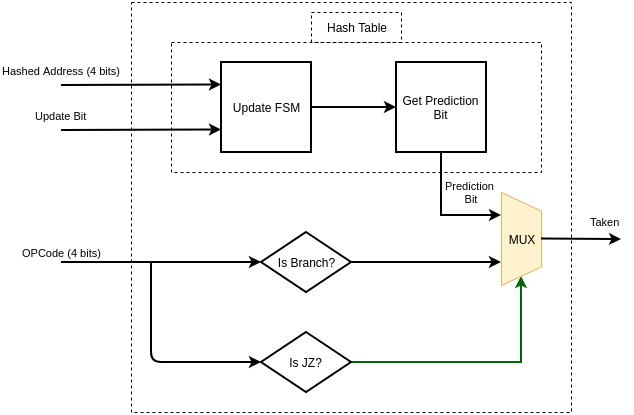
\includegraphics[width=0.8\textwidth]{images/bpu.png}
    \caption{Branch Prediction Unit Diagram}
    \label{fig:bpu}
\end{figure}

\subsection{Inputs}
\begin{itemize}
    \item Hashed Address (4 bits)
    \item Update Bit (1 bit): \emph{Taken or Not}  to update FSM
    \item OPcode (4 bits)
\end{itemize}

\subsection{Outputs}
\begin{itemize}
    \item Taken (1 bit): predict whether the branch taken or not
\end{itemize}

\subsection{Logic}
\begin{itemize}
    \item Updates the FSM corresponding to the hashed address.
    \item Checks whether the OPCode is of a conditional branch instruction.
    \item Outputs the prediction bit \emph{(Taken or Not)} accordingly.
\end{itemize}

\section{Branch Address Unit}
Figure \ref{fig:bau} shows the branch address unit.
\begin{figure}[hp]
    \centering
    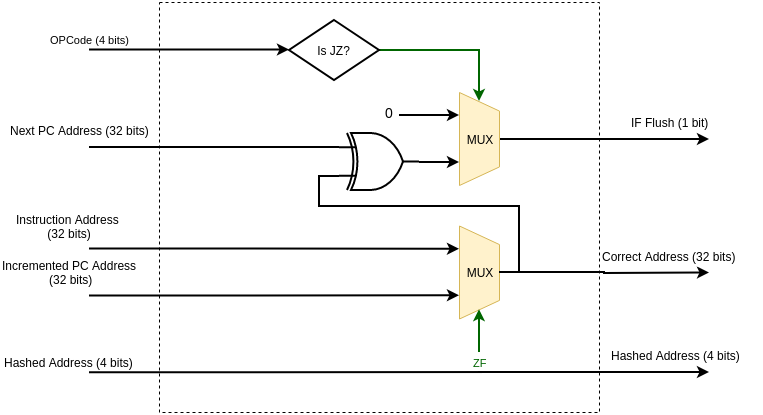
\includegraphics[width=0.8\textwidth]{images/bau.png}
    \caption{Branch Address Unit Diagram}
    \label{fig:bau}
\end{figure}

\subsection{Inputs}
\begin{itemize}
    \item Next PC Address (32 bits)
    \item Instruction Address (32 bits)
    \item Incremented PC Address (32 bits)
    \item Hashed Address (4 bits)
    \item OpCode (4 bits)
    \item CCR (3 bits)
\end{itemize}

\subsection{Outputs}
\begin{itemize}
    \item IF Flush (1 bit)
    \item Branch Address (32 bits)
    \item Feedback Hashed Address (4 bits)
\end{itemize}

\subsection{Logic}
\begin{itemize}
    \item Check if OpCode is of a conditional branch instruction, if true:
    \begin{itemize}
        \item Check whether PC Next Address is equal to Instruction Address
        \item If true:
        \begin{itemize}
            \item IF Flush = 0, Branch Address = Instruction Address
        \end{itemize}
        \item If false:
        \begin{itemize}
            \item IF Flush = 1, Branch Address = Instruction Address
        \end{itemize}
    \end{itemize}
    % TODO: what heppens if OpCode is not branch?
\end{itemize}

\section{Register File}
Figure \ref{fig:reg_file} shows the register file.
\begin{figure}[hp]
    \centering
    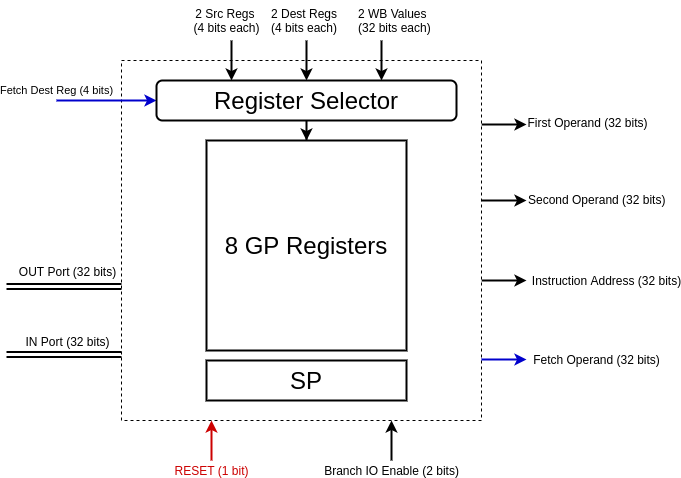
\includegraphics[width=0.8\textwidth]{images/reg_file.png}
    \caption{Register File Diagram}
    \label{fig:reg_file}
\end{figure}

\subsection{Registers}
All internal registers are 32bit in width. Each one has a 4bit address to select it, either for reading or writing.
\begin{itemize}
    \item 8 general purpose registers, addresses (0 to 7).
    \item Stack pointer (SP) register with address = 8.
\end{itemize}

\subsection{Inputs}
\begin{itemize}
    \item Dest Regs: 2$\times$4 bits (for destination selection)
    % TODO what is the address of io?
    \item SRC Regs: 2$\times$4 bits (for source selection)
    \item Fetch Reg: 4 bits (for fetch branch register selection)
    \item WB values: 2$\times$32 bits (for write back values)
    \item RESET 1 bit: async, clears all registers.
    \item BR\_IO\_ENBL: 2 bits (to determine whether the operation is IO or branch)\\
    00 = Do Nothing\\
    01 = In\\
    10 = Out\\
    11 = Branch\\
    \item IN Port: 32 bits (IO input port).
    % TODO: revise clock, is this right?
    \item CLK: input operations are in falling edge, while output operations are in rising edge.
\end{itemize}

\subsection{Outputs}
\begin{itemize}
    \item OP1: 32 bits (value of first operand (src0))
    \item OP2: 32 bits (value of second operand (src1))
    \item Fetch Value: 32 bits (value of branch address required by fetch)
    \item Instruction Address: 32 bits (value of branch address)
    \item OUT Port: 32 bits (IO output port)
\end{itemize}

\subsection{Logic}
The register selector acts like a decoder to select the required operation and the register on which the operation performed.

\section{ALU}

\subsection{Inputs}
\begin{itemize}
    \item ALUop: 4 bits (refer to ALU Operations below)
    \item Operands: 2$\times$32 bits (2 input operands)
\end{itemize}

\subsection{Outputs}
\begin{itemize}
    \item ALUout: 32 bits (operation result)
    \item CCR: 3 bits
\end{itemize}

\subsection{ALU Operations}
\begin{itemize}
    \item 0000 $-$ NOP $-$ (no operation)
    \item 0001 $-$ INC $-$ (first operand + 1)
    \item 0010 $-$ DEC $-$ (first operand - 1)
    \item 0011 $-$ ADD $-$ (first operand + second operand)
    \item 0100 $-$ SUB $-$ (first operand - second operand)
    \item 0101 $-$ AND $-$ (first operand \&\& second operand)
    \item 0110 $-$ OR $-$ (first operand $||$ second operand)
    \item 0111 $-$ NOT $-$ (!first operand)
    \item 1000 $-$ SHL $-$ (shift first operand to the left with the value of second operand)
    \item 1001 $-$ SHR $-$ (shift first operand to the right with the value of second operand)
    \item 1010 $-$ INC2 $-$ (first operand + 2)
    \item 1011 $-$ DEC2 $-$ (first operand - 2)
\end{itemize}

\subsection{Logic}
\begin{itemize}
    \item ALU performs the operation and changes the CCR accordingly.
    \item The input operands of the ALU are multiplexed between forwarded data and register data, with selectors from data forwarding unit.
\end{itemize}


\section{PC Navigator}
Figure \ref{fig:pc_nav} shows the PC Navigator.

\begin{figure}[hp]
    \centering
    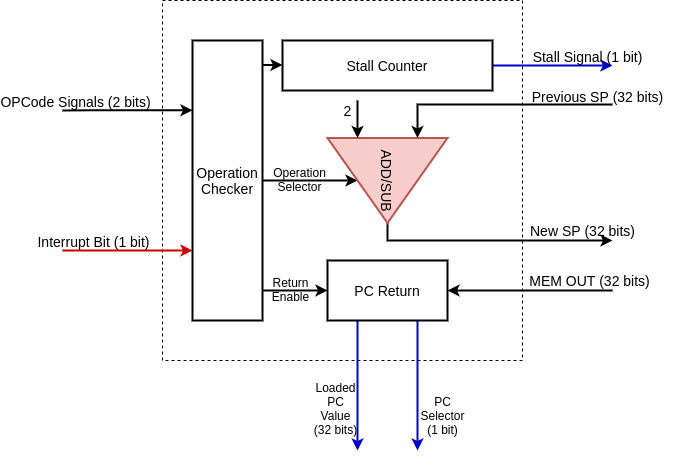
\includegraphics[width=0.8\textwidth]{images/pc_nav.png}
    \caption{PC Navigator Diagram}
    \label{fig:pc_nav}
\end{figure}

\subsection{Inputs}
\begin{itemize}
    \item Interrupt Bit (1 bit)
    \item OPCode Signals (2 bits): to check whether the operation is RET or RTI
    \item Previous SP (32 bits): to increment or decrement it correspondingly to access Data Memory
    \item MEM OUT (32 bits): loaded PC from memory
\end{itemize}

\subsection{Outputs}
\begin{itemize}
    \item Stall Signal (1 bit)
    \item New SP (32 bits)
    \item PC Selector (1 bit): to enable PC parallel load from Data Memory
    \item Loaded PC Value (32 bits)
\end{itemize}

\subsection{Logic}
\begin{itemize}
    \item The Operation Checker checks the OPCode Signals and Interrupt Bit to check whether the operation is RET, RTI or Interrupt and produces its signals accordingly:
    \begin{itemize}
        \item PC Return Enable is set.
        \item Counter is set to $0$ for RET, $1$ for RTI and $2$ for Interrupt.
        \item Operation Selector is issued to the Adder/Subtractor to change the value of SP.
    \end{itemize}
    \item Stall Counter counts the number of stalls produced by operation. It's set to $0$ for RET, $1$ for RTI and $2$ for Interrupt. It counts down a number of cycles and then release the stall.
    \item Adder/Subtractor is used to update the SP every stall cycle, to get the right data from the memory.
    \item PC Return issues a signal to the PC Control Unit to enable parallel load from data memory and passes the loaded PC value.
    \item RET doesn't stall any cycles, as it only loads PC value from data memory.
    \item RTI stall only one cycle, as it loads PC value from data memory and then loads CCR.
    \item Interrupt stall two cycles, as it loads PC value from data memory, pushes CCR into stack and then pushes PC into stack.
\end{itemize}
